

\section{Introduction}

\subsection{Motivation}
In this thesis we will apply integrals of motion as actions to Globular clusters (GC) to investigate possible signatures of intermediate-mass black holes (IMBH). 
\subsection{What is a globular cluster in the Milky Way?}
A GC is a collection of 10\(^6\) to 10\(^8\) stars which are spherically grouped. There are about 150 of them in the Milky Way (MW) halo. As some of the oldest stellar populations in the universe we can obtain much information about the evolution of the MW. Formerly seen as very simple system with only one stellar population and without rotation recent research revealed a much higher complexity of these systems. \color{red} nachlesen, wie das genau mit stellar populations und rotation und models ist \color{black}
\\In this color magnitude diagram (CMD) the visual magnitude is plotted against the B-V color. It's color coded by the mass of the star. A star's position can be interpreted as its evolution stage. Most of the stars are set in the main sequence. They fusion hydrogen in their cores. There are two main sequence lines one upon the other. These occur due to binary systems. These binary systems represent about \color{red} percentage \color{black} \% of the stars in the GC. The main sequence turn-off is depending on the age of the system and is used as indicator for such. Left to this turn off point there are so called blue stragglers \color{red} auch aktuell grade? was genau sind die? \color{black} Continuing from the turn off point there is the red giant branch consisting of stars still fusing hydrogen but only in a shell surrounding a degenerate helium core. They are inflated with a radius much higher than the main sequence stars but have only a very low temperature. At the end of the red giant branch lies the horizontal branch. Its stars have sun-like masses and burn helium in their core and hydrogen in a surrounding shell. In the lower left corner white dwarfs are located. They are stellar remnants which have burnt all of their resources. \color{red} nochmal über CMD durchlesen und alle branches erwähnen \color{black} In 3.1. we will compare the CMD to isochrones which describe the actual distribution of stars in the different stages for a given age and metallicity. 
\\In their centre GCs could contain an IMBH. These could be the missing link between stellar mass black holes and supermassive black holes (SMBH) as origin of the SMBH. Currently there are two different kinematic methods trying to detect IMBHs. As an example there are the unresolved/integrated IFU kinematics which result in a signature of an IMBH for NGC 6388 and resolved/discrete kinematics which don't yield IMBHs. \color{red} include graph of paolo's talk? \color{black} To get more certain methods we test if we can derive a signature of the IMBH by computing and comparing actions of the stars.


%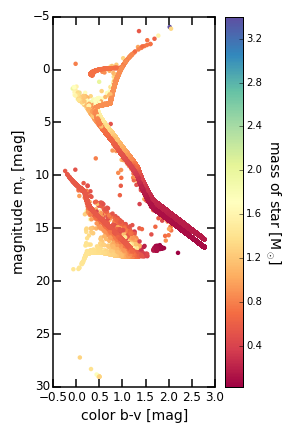
\includegraphics[width=\textwidth]{Plots/color_magnitude_diagram}
\subsection{Actions \& orbits}
Orbits contain all information about the potential of a system in their position and velocity coordinates following Newtons 2nd law. From the orbit distribution function we can draw inferences about the history of the system. Since there are many possible orbits but the stars are only on some of them questions are raised. How do they come on these special orbits? What do these orbits tell us about the evolution of the system? 
\\There are some examples when orbits enabled discoveries or confirmed them: 
\begin{itemize}
\item Seen from the earth Mars' position moves over the sky as a loop. That implies that the earth is not the centre of the universe!
\item Neptune/Uranus \color{red} noch mal nachlesen \color{black}
\item From rotation curves of galaxies we see that stars move faster than expected by mass of luminous matter. There has to be more matter interacting via gravitational forces. This has led to the theory of dark matter.
\item Mercury's orbit differs hugely from calculated Kepler orbit. This is because of its migrating pericentre. Due to the proximity to the sun gravitational forces are so strong that we need to apply general relativity.
\item The SMBH Sagittarius A*  was detected by observations of the orbits around the black hole and resulting mass calculations.
\end{itemize}
Some examples for orbit distribution functions are the asteroid belt, the distribution function of moons around planets which allows feedback connections to formation and bonding of different planet types and spiral galaxies where stars of different parts(thin disc, thick disc, bulge, halo) have different orbits (dynamical distinct) and different metallicity (chemical distinct).
\\\\
Actions are integrals of motion and are the distinct description of orbits. They are constant with time. Known for a long time they are extremly difficult to calculate. Actions of our solar system can be calculated easier since we know the potential. With nowadays supercomputers it's finally possible to compute actions of more complex and less explored systems.

